\documentclass[11pt]{report}

\usepackage[latin9]{inputenc}
\usepackage[T1]{fontenc}

\usepackage[spanish,es-nolayout,es-nodecimaldot]{babel}

\usepackage{makeidx}

\usepackage{multicol}

%\usepackage{arev}
%\usepackage{mathptmx}

\usepackage[sfmath]{kpfonts}
\renewcommand*\familydefault{\sfdefault}

\usepackage{amsmath,amssymb,amsthm,mathrsfs,bm,ifthen}

\usepackage{cancel}
\usepackage{soul}

\usepackage[dvipsnames,svgnames]{xcolor}
\usepackage{colortbl}
\usepackage{tikz}

\usepackage{pifont}
\usepackage{enumitem}
\usepackage{setspace}
\usepackage{longtable}

\usepackage{nextpage}

\usepackage{pst-eucl,pstricks-add}
\usepackage[framemethod=TikZ]{mdframed}

\usepackage{fancyhdr}
\usepackage{lastpage}

\usepackage[a4paper,top=2.5cm,bottom=2.5cm,left=3.0cm,right=3.0cm]{geometry}

\usepackage[bookmarks,colorlinks,linkcolor=red]{hyperref}

%\usepackage{materialjc,macmatjc}  \\paquetes de JC

\setstretch{1.2}
%\setstretch{1.04}

\parskip 0.7\baselineskip
%\parskip 0.3\baselineskip

\parindent 0pt

\allowdisplaybreaks

\setulcolor{red}

\bibliographystyle{plain}

%%%%\tccbjc: tikz caja centrada borde jc
%%%% #1: color de fondo, #2: color del borde, #3: color del texto
%%%% #4: separaci�n interna, #5: ancho de la caja, #6: el texto
\newcommand{\tccbjc}[6]{%
\begin{center}
\begin{tikzpicture}[rounded corners]
\draw (0,0) node[text justified, text width=#5, fill = #1, inner sep = #4]
{\color{#3}
#6};
\draw[color = #2, rounded corners] (current bounding box.south west) rectangle
(current bounding box.north east);
\end{tikzpicture}
\end{center}
}
%%

\renewcommand{\CancelColor}{\red}

%%%%
%%  Definiciones provisionales
%%%%
\newcommand{\titleexample}[1]{\textcolor{red}{\small{\textsc{#1}}}}

\definecolor{PD}{named}{OliveGreen}
\newcommand{\pd}[1]{\textcolor{PD}{#1}}

%%% \enunciado
\newcommand{\enunciado}[1]{\textit{\color{OliveGreen} #1}}

%%% \retroalimentacion
\newcommand\retroalimentacion{\textsc{\textbf{\textcolor{red}{Retroalimentaci\'on}}}}

%%% \demostracion
\newcommand\demostracion{\textsc{\textbf{\textcolor{red}{Demostraci\'on}}}}

%%% \finretroalimentacion
\newcommand\finretroalimentacion{\hfill\textsc{\textbf{\textcolor{red}{Fin de la retroalimentaci\'on}}}}

%%% \finadvertencia
\newcommand\finadvertencia{\hfill\textbf{\textcolor{red}{Fin de la advertencia}}}

%%% \finatencion
\newcommand\finatencion{\hfill\textbf{\textcolor{red}{Fin de la atenci\'on}}}

%%% \listapropiedades
%\newcommand\listapropiedades{\texttt{\textcolor{DarkOrchid}{Lista de propiedades}}}

%%% \listapropiedades
\newcommand{\listapropiedades}[1]{%
  \texttt{\textcolor{DarkOrchid}{#1}}%
}

%%% \justificacion
\newcommand{\justificacion}[1]{%
  \texttt{\textcolor{ForestGreen}{#1}}%
}

%%% \aqui
\newcommand{\aqui}[1]{%
  \rnode{#1}{\phantom{=}}%
}

%%%\une
\newcommand{\une}[3]{%
  \ncline[linecolor=#3]{->}{#1}{#2}%
}
%

%%%\tr
\newcommand{\tr}[1]{%
  \textcolor{red}{#1}%
}
%

%%%\borrador
\def\borrador{%draft%
}
%

%%%\borradorr
\def\borradorr{%draft%
}
%

%%%%\potencia
\newcommand{\potencia}[2]{%
  \overset{#2 \text{ veces}}{\overbrace{#1\cdot #1 \cdots #1}}
}
%

\mdfdefinestyle{definitionstyle}{%
  frametitlefontcolor=black,linecolor=DarkCyan,outerlinewidth=2pt,innerlinewidth=0pt%
  frametitlerule=true,%
  roundcorner=5pt,%
  frametitlebackgroundcolor=DarkCyan!75,
  innertopmargin=2.5\topskip,innerbottommargin=1.5\topskip
  innerleftmargin=12pt,innerrightmargin=12pt,
  skipabove=0.5\baselineskip,
  skipbelow=0.5\baselineskip
  }
\mdtheorem[style=definitionstyle]{definition}{Definici\'on}
\mdtheorem[style=definitionstyle]{concepts}{Conceptos primitivos o fundamentales}

\mdfdefinestyle{exercisestyle}{%
  frametitlefontcolor=black,linecolor=Orange,outerlinewidth=2pt,innerlinewidth=0pt%
  frametitlerule=true,%
  roundcorner=5pt,%
  frametitlebackgroundcolor=Orange!75,
  innertopmargin=2.75\topskip,innerbottommargin=1.75\topskip
  skipabove=\baselineskip,
  skipbelow=0.5\baselineskip
  }
\mdtheorem[style=exercisestyle]{exercise}{Ejercicio}
\mdtheorem[style=exercisestyle]{exercises}{Ejercicios}

\mdfdefinestyle{principlestyle}{%
  frametitlefontcolor=black,linecolor=Olive,outerlinewidth=2pt,innerlinewidth=0pt%
  frametitlerule=true,%
  roundcorner=5pt,%
  frametitlebackgroundcolor=Olive!75,
  innertopmargin=1.75\topskip,innerbottommargin=1.5\topskip
  innerleftmargin=12pt,innerrightmargin=12pt,
  skipabove=0.5\baselineskip,
  skipbelow=0.5\baselineskip
  }
\mdtheorem[style=principlestyle]{principle}{Principio}
\mdtheorem[style=principlestyle]{principles}{Principios}
\mdtheorem[style=principlestyle]{axiom}{Axioma}

\mdfdefinestyle{propertystyle}{%
  frametitlefontcolor=black,linecolor=DarkOrchid,outerlinewidth=2pt,innerlinewidth=0pt%
  frametitlerule=true,%
  roundcorner=5pt,%
  frametitlebackgroundcolor=DarkOrchid!75,
  innertopmargin=2\topskip,innerbottommargin=1.25\topskip
  innerleftmargin=12pt,innerrightmargin=12pt,
  skipabove=0.5\baselineskip,
  skipbelow=0.5\baselineskip
  }
%\mdtheorem[style=propertystyle]{property}{Propiedad}
\mdtheorem[style=propertystyle]{property}{Teorema}

\mdfdefinestyle{examplestyle}{%
  frametitlefontcolor=black,linecolor=Yellow,outerlinewidth=2pt,innerlinewidth=0pt%
  frametitlerule=true,%
  roundcorner=5pt,%
  frametitlebackgroundcolor=Yellow!50,
  innertopmargin=2\topskip,innerbottommargin=1.25\topskip
  skipabove=0.5\baselineskip,
  skipbelow=0.5\baselineskip
  }
\mdtheorem[style=examplestyle]{example}{Ejemplo}
\mdtheorem[style=examplestyle]{examples}{Ejemplos}

\mdfdefinestyle{procedurestyle}{%
  frametitlefontcolor=black,linecolor=Orange,outerlinewidth=2pt,innerlinewidth=0pt%
  frametitlerule=true,%
  roundcorner=5pt,%
  frametitlebackgroundcolor=Orange!50,
  innertopmargin=2\topskip,innerbottommargin=1.25\topskip
  skipabove=0.5\baselineskip,
  skipbelow=0.5\baselineskip
  }
\mdtheorem[style=procedurestyle]{procedure}{Procedimiento}

\mdfdefinestyle{countingstyle}{%
  linecolor=DarkOrange,outerlinewidth=2pt,innerlinewidth=0pt%
  frametitlerule=true,%
  roundcorner=5pt,%
  frametitlebackgroundcolor=DarkOrange!75,
  innertopmargin=2\topskip,innerbottommargin=1.25\topskip
  skipabove=0.5\baselineskip,
  skipbelow=0.5\baselineskip
  }
\mdtheorem[style=countingstyle]{counting}{T\'ecnica de conteo}

%#1: n�mero de objetos seleccionado
%#2: total de objetos
\newcommand\variaciones[2]{V_{#1}^{#2}}
\newcommand\variacionesR[2]{VR_{#1}^{#2}}
\newcommand\combinaciones[2]{C_{#1}^{#2}}
\newcommand\combinacionesR[2]{CR_{#1}^{#2}}
\newcommand\distribuciones[2]{D_{#1}^{#2}}

%2015 04 06
%%% \recurso{#1}{#2}{#3}
%%% #1: Tipo de recurso; p.e., "Libro electr\'onico", "Libro electr\'onico con animaciones incrustadas", etc\'etera
%%% #2: Nombre del recurso
%%% #3: Etiqueta

\newcommand\recurso[3][]{%
  \begin{center}
  \ifthenelse{\equal{#1}{}}{}{\label{#1}}
  \bfseries\large\color{azulCLAVEMAT}
  \underline{#2}:

  \underline{#3}
  \end{center}%
}

\def\espacio{\quad \textcolor{Red}{\Box} \quad }
%%% \begin{animacioni}[#1] ... \end{animacioni}
%%% #1: Opcional. Para texto alternativo del encabezado de la tercera columna: "Amimaci�n en pantalla$^\ast$

\newenvironment{animacioni}[1][Imagen / texto referencial en pantalla o animaci�n en pantalla]{%
  \begingroup
    \begin{center}
      \small
      \setlength\extrarowheight{4pt}
      \begin{longtable}{|>{\centering\hspace{0pt}}m{0.1\textwidth}%
                        |>{\raggedright\hspace{0pt}}m{0.415\textwidth}%
                        |>{\raggedright\hspace{0pt}}m{0.485\textwidth}|}\hline
        \textbf{Secuencia} & \centering\textbf{Texto para locuci\'on} & \centering\hspace{0pt}\parbox{0.48\textwidth}{\textbf{#1}} \tabularnewline\hline
        \endfirsthead
        \hline\textbf{Secuencia} & \centering\textbf{Texto para locuci\'on} & \centering\hspace{0pt}\parbox{0.48\textwidth}{\textbf{#1}} \tabularnewline\hline
        \endhead
        \multicolumn{3}{r}{\textit{Contin\'ua en la p\'agina siguiente}}
        \endfoot
        \hline
        \endlastfoot}% Fin de begdef
  {%
      \end{longtable}
    \end{center}
  \endgroup}% Fin de enddef

\newcommand\expositor{\texttt{Juan Carlos Trujillo} exponiendo}

\tolerance=1
\emergencystretch=\maxdimen
\hyphenpenalty=10000
\hbadness=10000

\newcommand\headerle[3]{%
  \thispagestyle{empty}

  \vspace{7.5\baselineskip}
  \begin{center}
    \psframebox[border=0pt,linecolor=white,fillstyle=solid,fillcolor=Red]{\textcolor{white}{\LARGE{SUBSECCI\'ON #1}}}
    \\
    \psframebox[border=0pt,linecolor=white,fillstyle=solid,fillcolor=black]{\textcolor{white}{\large{#2}}}
  \end{center}

  \vspace{10\baselineskip}
  \begin{center}
  \Huge
  \textcolor{Red}{#3}
  \end{center}

  \newpage

  \setcounter{page}{1}
}

\newcommand\headerlg[2]{%
  \thispagestyle{empty}

  \vspace{7.5\baselineskip}
  \begin{center}
    \psframebox[border=0pt,linecolor=white,fillstyle=solid,fillcolor=Red]{\textcolor{white}{\LARGE{SECCI\'ON #1}}}
  \end{center}

  \vspace{10\baselineskip}
  \begin{center}
  \Huge
  \textcolor{Red}{#2}
  \end{center}

  \newpage

  \setcounter{page}{1}
}

%%%\underlabel{#1}{#2}
\newcommand\underlabel[2]{%
  \underset{\footnotesize{\text{#2}}}{\underbrace{#1}}
}%

%%%\overlabel{#1}{#2}
\newcommand\overlabel[2]{%
  \overset{\footnotesize{\text{#2}}}{\overbrace{#1}}
}%

\definecolor{azulCLAVEMAT}{rgb}{0.04,0.41,0.75}


%%%\entrega{#1}
\newcommand\entrega[1]{%
  \textcolor{red}{\ (fecha de entrega: #1)}
}
%

%%% \plano
\newcommand\plano{\mathscr{P}}
%

%%% \figura
\newcommand\figura{\mathscr{F}}
%

%%% \figura
\newcommand\semiplano{\mathscr{S}}
%

%%% \recta{#1}{#2}
\newcommand\recta[2]{%
  \overset{\longleftrightarrow}{#1#2}
}
%

%
\newcommand\entre[3]{%
  #1\!-\!#2\!-\!#3%
}

%%%%
\newcommand\segmento[2]{\overline{#1#2\,}}

%%%%
\newcommand\lado[2]{\overline{#1#2\,}}

%%%%
\newcommand\rayo[2]{\overrightarrow{#1#2}}

%%%
\newcommand\angulo[3]{\angle #1#2#3}

%%%
\newcommand\mangular[3]{\textrm{m}\,\angle #1#2#3}

%%%
\newcommand\mangularv[1]{\textrm{m}\,\angle #1}

%%%%
\newcommand\correspondencia[2]{%
  \triangle #1 \longleftrightarrow \triangle #2%
}

%%%%
\newcommand\congruencial[2]{%
  \overline{#1\,} \cong \overline{#2\,}%
}
%%%%
\newcommand\congl[2]{%
  \overline{#1\,} \cong \overline{#2\,}%
}

%%%%
\newcommand\congruenciaa[2]{%
  \angle #1 \cong \angle #2%
}
%%%%
\newcommand\conga[2]{%
  \angle #1 \cong \angle #2%
}

%%%%
\newcommand\congruenciat[2]{%
  \triangle #1 \cong \triangle #2%
}
%%%%
\newcommand\congt[2]{%
  \triangle #1 \cong \triangle #2%
}

%%%%
\newcommand\perpra[2]{%
  \overrightarrow{#1} \perp \overrightarrow{#2}
}

%%%%
\newcommand\perpre[2]{%
  \overset{\longleftrightarrow}{#1} \perp \overset{\longleftrightarrow}{#2}
}

%%%%
\newcommand\perps[2]{%
  \lado{#1}\perp\lado{#2}
}

%%%%
\newcommand\perprer[2]{%
  \recta{#1}\perp\rayo{#2}
}

%%%%
\newcommand\perprar[2]{%
  \rayo{#1}\perp\recta{#2}
}

%%%%
\newcommand\perpras[2]{%
  \rayo{#1}\perp\lado{#2}
}
%%%%
\newcommand\perpsra[2]{%
  \lado{#1}\perp\rayo{#2}
}

%%%%
\newcommand\perpres[2]{%
  \overset{\longleftrightarrow}{#1}\perp\overline{#2\,}
}
%%%%
\newcommand\perpsre[2]{%
  \lado{#1}\perp\recta{#2}
}

%%%%
\newcommand\semejanza[2]{%
  \triangle #1 \simeq \triangle #2
}

\newcommand\fA{\textcolor{ForestGreen}{\texttt{S}}}
\newcommand\fC{\textcolor{ForestGreen}{\texttt{D}}}
\newcommand\fG{\textcolor{ForestGreen}{\texttt{P}}}
\newcommand\fN{\textcolor{ForestGreen}{\texttt{N}}}
\newcommand\fO{\textcolor{ForestGreen}{\texttt{O}}}
\newcommand\rf[2]{\textcolor{ForestGreen}{\texttt{#1#2}}}
\newcommand\pf[2]{\textcolor{ForestGreen}{(\texttt{#1, #2})}}
\newcommand\rfe[2]{\textcolor{Maroon}{\texttt{#1#2}}}
\newcommand\rt[3]{\textcolor{ForestGreen}{\texttt{#1#2#3}}}
\newcommand\rc[4]{\textcolor{ForestGreen}{\texttt{#1#2#3#4}}}
\newcommand\ri[5]{\textcolor{ForestGreen}{\texttt{#1#2#3#4#5}}}

\begin{document}
\nocite{*}

\title{}
\author{Elaboraci\'on de contenidos: Eduardo Arias}
\date{}
%\maketitle
\newpage\cleartooddpage[\thispagestyle{empty}]

\def\chaptername{Secci\'on}

%\tableofcontents
\cleartooddpage[\thispagestyle{empty}]

%%%%%%%%%%%%%%%%%%%%%%%%%%%%%%%%%%%%%%
\newcommand{\poruno}[1]{\dfrac{#1}{#1}}
    \chapter*{Definiciones previas}
    \begin{definition}
    Dadas dos funciones \(f\) y \(g\) se definen las operaciones siguientes:
    \begin{enumerate}
    \item su \textbf{suma} como 
    \[
    (f+g)(x)=f(x)+g(x)
    \]
    \item su \textbf{diferencia} como
    \[
    (f-g)(x)=f(x)-g(x)
    \]
    \item su \textbf{producto} como
    \[
    (f\cdot g)(x)=f(x)\cdot g(x)
    \]
    \item su \textbf{cociente} como
    \[
    (f/ g)(x)=f(x)/g(x)\qquad g(x)\neq 0
    \]
    \end{enumerate}
    \end{definition}
    %%%%% ejemplo de operaciones entre funciones
    Por ejemplo, demos dos funciones \(f(x)=x^2\) y \(g(x)=\frac{1}{x^2-1}.\) Operemos un poco con estas dos funciones:\\
    \begin{itemize}
    	\item Sumemos \(f+g\)
    	\begin{align*}
    	(f+g)(x)&=f(x)+g(x)\\
    	&=x^2+\dfrac{1}{x^2-1}\\
    	&=\dfrac{x^4-x^2+1}{x^2-1}
    	\end{align*}
    	
	    \item Restemos \(f-g\)
	    \begin{align*}
	    (f-g)(x)&=f(x)-g(x)\\
	    &=x^2-\dfrac{1}{x^2-1}\\
	    &=\dfrac{x^4-x^2-1}{x^2-1}
	    \end{align*}
	    
	    \item Multipliquemos ambas funciones
	    \begin{align*}
	    (f\cdot g)(x)&=f(x)\cdot g(x)\\
	    &=x^2\cdot\dfrac{1}{x^2-1}\\
	    &=\dfrac{x^2}{x^2-1}
	    \end{align*}
	    
	    \item Dividamos ambas funciones
	    \begin{align*}
	    (f/g)(x)&=\dfrac{f(x)}{g(x)}\\
	    &=x^2\cdot(x^2-1)\\
	    &=x^4-x^2
	    \end{align*}
    \end{itemize}
    Adem\'as, si quieren encontrar el dom\'inio de la funci\'on obtenida solo deber\'ian intersecar los dominios de las funciones con las que operaron. Por ejemplo sabemos que el dom\'inio de la funci\'on \(f(x)=x^2\) es \(\mathbb{R}\) y de la funci\'on \(g(x)=\frac{1}{x^2-1}\) es \(\mathbb{R}-\{-1,1\},\) ahora intersecando ambos dominios obtienen el dom\'inio de la funci\'on \(f\cdot g\) que es \(\mathbb{R}\cap\left(\mathbb{R}-\{-1,1\}\right)=\mathbb{R}-\{-1,1\}.\)\newline
    
    %%%%%%%%% DEFINICION FUNCION COMPUESTA
    \begin{definition}
     Dadas dos funciones \(f\) y \(g,\) la funci\'on compuesta denotada por \(f\circ g,\) est\'a definida por
     \[
     (f\circ g)(x)=f(g(x)).
     \]
    \end{definition}
    
    %%%%%%%%%%%%% FUNCION COMPUESTA
    %%%%%%%%%%%%%%%% MEJORAR EL GR�FICO
    \begin{center}
		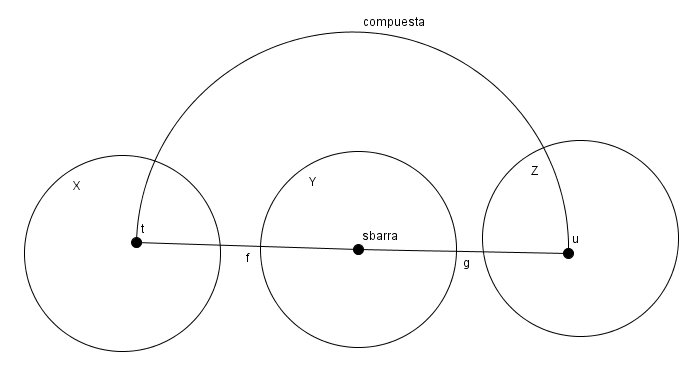
\includegraphics[scale=0.7]{recursos_graficos/funcion_compuesta}
    \end{center}
    
    %%%%%%%%%%% EJERCICIOS DE 
    \begin{exercise}
    Determine el dominio de la funci\'on resultante
    \begin{enumerate}
    \item \(f+g\)
    \item \(f-g\)
    \item \(f\cdot g\)
    \item \(f/g\)
    \item \(g/f\)
    \end{enumerate}
    si \(f(x)=\sqrt{x}\) y \(g(x)=x^2+1.\)
    \end{exercise}
    
    \begin{example}
    La funci\'on Raz\'iz Cuadrada est\'a definida de reales no negativos (reales positivos uni\'on el cero) en reales no negativos, as\'i
    de la funci\'on \(f\) obtenemos una restricci\'on que es \(x\geq 0,\) por ende el dom\'inio de la funci\'on \(f\) es \([0;+\infty[.\) Por otro lado, la funci\'on \(g\) es un polin\'omio, por lo cu\'al su dom\'inio es todos los reales.\newline
    
    Ahora, para encontrar el dom\'inio de la funci\'on \(f+g\) debemos intersecar ambos dom\'inios, es decir, que el dom\'inio es \([0;+\infty[.\)
    
    Para la funci\'on \(f-g\) es el mismo dom\'inio, pues
    \begin{align*}
    (f-g)(x)&=f(x)-g(x)\\
    &=-1*g(x).
    \end{align*}
    Al igual que para la suma y la diferencia, el dom\'inio es el mismo pues
    \begin{align*}
    (f\cdot g)(x)&=f(x)\cdot g(x)\\
    &=\sqrt{x}\;(x^2+1)\\
    &=x^{\frac{3}{2}}+\sqrt{x}
    \end{align*}
    
    
    Ahora, para %%%%%%%%%%%%% Ya esta en el Texto.tex
    \end{example}
    
    
    
    \begin{definition*}[Funci\'on par e impar]
    \begin{enumerate}
    \item Una funci\'on \(f\) se dice par cuando para cada \(x\) en el dominio de \(f\)
    \[
    f(-x)=f(x)
    \]
    \item Una funci\'on \(f\) se dice impar cuando para cada \(x\) en el dominio de \(f\)
    \[
    f(-x)=-f(x)
    \]
    \end{enumerate}
    \end{definition*}
    
	\chapter{L\'imites}
	%%%% DEFINICION DE L�MITE DE UNA SUCESI�N	
	\begin{definition}
		\(L\) se dice que es el l\'imite de una sucesi\'on \(x_1,x_2,x_3,\cdots,x_n,\cdots\) si, para todo \(\epsilon>0\) existe un n\'umero \(N\) en los naturales tal que
		\[\left|x_n-L\right|<\epsilon\quad\text{ para }\quad n>N.\]
	\end{definition}
	
	%%%% DEFINICION DE L�MITE
	\begin{definition}
		Sea \(f\) una funci\'on definida en alg\'un intervalo que contenga a \(a,\) excepto posiblemente en en \(a\) mismo. El l\'imite se define como \[(\forall\varepsilon>0)\,(\exists\delta>0)\,(0<\left|x-a\right|<\delta\Rightarrow\left|f(x)-L\right|<\varepsilon)\]
	\end{definition}
	

%%%%%%%%%%%%%%%%%%%%% TEOREMA propiedades de l�mites
	\begin{property}
		Sean \(f_1\) y \(f_2\) dos funciones, si existen \(\lim\limits_{n\to+\infty}f_1(x)\) y \(\lim\limits_{n\to+\infty}f_2(x)\) entonces se cumplen las siguientes propiedades:
		\begin{enumerate}
			\item \(\lim\limits_{n\to+\infty}\left[f_1(x)+f_2(x)\right]=\lim\limits_{n\to+\infty}f_1(x)+\lim\limits_{n\to+\infty}f_2(x)\)						\item \(\lim\limits_{n\to+\infty}\left[f_1(x)\cdot f_2(x)\right]=\lim\limits_{n\to+\infty}f_1(x)\cdot\lim\limits_{n\to+\infty}f_2(x)\)
			\item \(\lim\limits_{n\to+\infty}\left[\dfrac{f_1(x)}{f_2(x)}\right]=\dfrac{\lim\limits_{n\to+\infty}f_1(x)}{\lim\limits_{n\to+\infty}f_2(x)}\quad\text{si }\lim\limits_{n\to+\infty}f_2(x)\neq 0.\)
		\end{enumerate}
	\end{property}


\begin{property}
	Sea \(f\) una funci\'on,
	\[\lim\limits_{x\to a}f(x)=L\qquad\mbox{s� y solo si}\qquad\lim\limits_{x\to a^{-}}f(x)=L=\lim\limits_{x\to a^{+}}f(x)=L\]
\end{property}

\begin{property*}[Teorema del Sanduche]
	Sean \(f,\) \(g\) y \(h(x)\) dos funciones tales que \(f(x)\leq g(x)\leq h(x)\) cuando \(x\) tiende a \(a\) (excepto posiblemente en \(a\)), y adem�s
	\[\lim\limits_{x\to a}f(x)=\lim\limits_{x\to a}h(x)=L,\]
	entonces
	\[\lim\limits_{x\to a}g(x)=L.\]
\end{property*}

%%%%%%%%%%%%%%%%%%% EJERCICIOS DE LIMITES POR DEFINICION	
		\begin{exercise}
			Demostrar por la definici\'on de l\'imite que
			\[
			\lim\limits_{x\to 2}{\dfrac{x^2-4}{x-2}}=4.
			\]
		\end{exercise}
		\begin{example}
			Aqu\'i la funci\'on \(f(x)=\frac{x^2-4}{x-2}\) no est\'a definida en el punto \(x=2.\)\newline
			
			Es necesario demostrar que, tomando un \(\varepsilon > 0\) arbitrario encontraremos un \(\delta >0\) que cumpla la desigualdad
			\[\left|\dfrac{x^2-4}{x-2}\right|<\varepsilon,\]
			con la condici\'on que \(\left|x-2\right|<\delta.\) Pero para \(x\neq 2,\) la desigualdad anterior es equivalente a 
			\begin{align*}
			\left|\dfrac{(x-2)(x+2)}{x-2}-4\right|&=\left|(x+2)-4\right|\\ 
			&<\varepsilon.
			\end{align*}
			
			As\'i pues, siendo \(\varepsilon\) arbitrario, y tomando \(\delta=\varepsilon\) se cumplen las desigualdades anteriores.\newline
			
			Esto significa que el l\'imite de \(f(x)\) es 4, cuando \(x\to 2.\)
		\end{example}
		\begin{exercise}[L\'imite al infinito]
			Demostremos que 
			\[
			\lim\limits_{x\to+\infty}{\dfrac{x+1}{x}}=1
			\]
		\end{exercise}
		\begin{example}
			Como se puede observar
			\[
			\dfrac{x+1}{x}=1+\dfrac{1}{x},
			\]
			por lo cual podemos utilizar esto en el l\'imite.\newline
			
			Ahora, necesitamos demostrar que siendo \(\varepsilon>0\) se cumplir\'a la desigualdad
			\begin{equation}
			\left|\left(1+\dfrac{1}{x}\right)-1\right|<\varepsilon,
			\end{equation}
			siempre que \(\left|x\right|>N,\) donde \(N>0\) depende de nuestro \(\varepsilon.\)\newline
			%%%%%%%%%%%%%%% Verificar el n�mero de la desigualdad
			Operando la desigualdad (1.3) obtenemos que
			
			\begin{equation}
			\begin{aligned}
			\left|\frac{1}{x}\right|&<\varepsilon,
			\end{aligned}
			\end{equation}
			
			que es lo mismo que
			\begin{equation}
			\begin{aligned}
			\left|x\right|&>\frac{1}{\varepsilon}\\
			&=N.
			\end{aligned}
			\end{equation}
			Esto significa que \(\displaystyle\lim\limits_{x\to+\infty}\left(1+\frac{1}{x}\right)=\displaystyle\lim\limits_{x\to+\infty}\frac{x+1}{x}=1.\)
		\end{example}
		
%%%%%%%%%%%%% LIMITES DE SUCESIONES
	
	\begin{exercise}
	Hallar los l\'imites de las sucesiones
	\begin{enumerate}
	\item \(1,-\frac{1}{2},\frac{1}{3},\dots,(-1)^{n-1}\frac{1}{n},\dots\)
	\item \(\frac{2}{1},\frac{4}{3},\frac{6}{5},\dots,\frac{2n}{2n+1},\dots\)
	\item \(\sqrt{2},\sqrt{2\sqrt{2}},\sqrt{2\sqrt{2\sqrt{2}}},\dots\)
	\end{enumerate}
	\end{exercise}
	
	\begin{example}
	\begin{enumerate}
	\item Veamos la expresi\'on \(x_n=(-1)^{n-1}\frac{1}{n}\) en dos casos, si \(n\) es par tenemos que
	
	\[\lim\limits_{n\to +\infty}{x_n}=\lim\limits_{n\to +\infty}{-\frac{1}{n}}=0.\]
	
	Ahora veamos el caso en que \(n\) es impar, as\'i se tiene que
	
	\[\lim\limits_{n\to +\infty}{x_n}=\lim\limits_{n\to +\infty}{(-1)^{n-1}\frac{1}{n}}=\lim\limits_{n\to+\infty}{\frac{1}{n}}=0.\]
	
	\item Notemos como \(x_n=\frac{2n}{2n+1},\) entonces 
	\[\lim\limits_{n\to+\infty}\frac{2n}{2n+1}=\lim\limits_{n\to+\infty}\frac{2}{2+\frac{1}{n}}=1.\]
	\item Para esta sucesi\'on veamos como son uno a uno sus t\'erminos:\newline
	
	\begin{equation*}
	\begin{array}{lclclcl}
	 a_1&=&\sqrt{2}&=&2^{\frac{1}{2}}\\
	 a_2&=&\sqrt{2\sqrt{2}}&=&2^{\frac{1}{2}}\cdot 2^{\frac{1}{4}}&=&2^{\frac{1}{2}+\frac{1}{4}}\\
	 a_3&=&\sqrt{2\sqrt{2\sqrt{2}}}&=&2^{\frac{1}{2}+\frac{1}{4}}\cdot 2^{\frac{1}{8}}&=&2^{\frac{1}{2}+\frac{1}{4}+\frac{1}{8}}\\
	 \vdots\\
	 a_n&=&2^{\frac{1}{2}(1+\frac{1}{2}+\frac{1}{2^2}+\cdots+\frac{1}{2^{n+1}})}\\
	\end{array}
	\end{equation*}
		en donde la expresi\'on 
	\[1+\frac{1}{2}+\frac{1}{2^2}+\cdots+\frac{1}{2^{n+1}}\]
	es una prograsi\'on geom\'etrica, con lo cu\'al obtenemos que
	\[a_n=2^{\frac{1}{2}\cdot 2(1-\frac{1}{2^n})},\]
	y as\'i, se tiene que
	\[\lim\limits_{n\to+\infty}{a_n}=\lim\limits_{n\to+\infty}{2^{\frac{1}{2}\cdot 2(1-\frac{1}{2^n})}}=2.\]

	\end{enumerate}
	\end{example}
	
	%%%%%%%%%%%%%% LIMITES DE SUCESIONES
	
	\begin{exercise}
	Halle los l\'imites de:
	\begin{enumerate}
	\item \(\lim\limits_{n\to+\infty}\left(\frac{1}{n^2}+\frac{2}{n^2}+\cdots+\frac{n-1}{n^2}\right)\)
	\item \(\lim\limits_{n\to+\infty}{\frac{(n+1)(n+2)(n+3)}{n^3}}.\)
	\item \(\lim\limits_{n\to+\infty}{\left(\sqrt{n+1}-\sqrt{n}\right).}\)
	\item \(\lim\limits_{n\to+\infty}{\frac{n\sin(n!)}{n^2+1}}.\)
	\end{enumerate}
	\end{exercise}
	%%%%%%%%%%%%%%% EXPLICACI�N DEL PORQUE LA RESOLUCION DE LOS EJERCICIOS
	Comencemos recordando que
	\[\displaystyle\sum_{i=1}^{n}{i}=\dfrac{n(n+1)}{2}.\]
	Adem�s, conocemos que el recorrido de la funci\'on Seno y Coseno es \([-1;1].\)
	
	\begin{example}
\begin{enumerate}
\item Notemos a \(x_n=\left(\frac{1}{n^2}+\frac{2}{n^2}+\cdots+\frac{n-1}{n^2}\right),\) ahora
\begin{align*}
\lim\limits_{n\to+\infty}{x_n}&=\lim\limits_{n\to+\infty}\left(\frac{1}{n^2}+\frac{2}{n^2}+\cdots+\frac{n-1}{n^2}\right)\\
&=\lim\limits_{n\to+\infty}\dfrac{n(n-1)}{2n^2}\\
&=\lim\limits_{n\to+\infty}{\dfrac{n^2-n}{2n^2}}\\
&=\lim\limits_{n\to+\infty}{\dfrac{1-\frac{1}{n}}{2}}\\
&=\frac{1}{2}.
\end{align*}

\item Llamemos \(x_n\) a la expresi\'on \(\frac{(n+1)(n+2)(n+3)}{n^3}.\) Calculemos el l\'imite
\begin{align*}
\lim\limits_{n\to+\infty}{x_n}&=\lim\limits_{n\to+\infty}{\frac{(n+1)(n+2)(n+3)}{n^3}}\\
&=\lim\limits_{n\to+\infty}{\left(\frac{n+1}{n}\right)\left(\frac{n+2}{n}\right)\left(\frac{n+3}{n}\right)}\\
&=\lim\limits_{n\to+\infty}{\left(1+\dfrac{1}{n}\right)\left(1+\dfrac{2}{n}\right)\left(1+\dfrac{3}{n}\right)}\\
&=1.
\end{align*}
\item Notemos como \(x_n\) a a expresi\'on \(\sqrt{n+1}-\sqrt{n}.\)
Arhora,
\begin{align*}
\lim\limits_{n\to+\infty}{x_n}&=\lim\limits_{n\to+\infty}{\sqrt{n+1}-\sqrt{n}}\\
&=\lim\limits_{n\to+\infty}{\left(\sqrt{n+1}-\sqrt{n}\right)\dfrac{\sqrt{n+1}+\sqrt{n}}{\sqrt{n+1}+\sqrt{n}}}\\
&=\lim\limits_{n\to+\infty}{\dfrac{1}{\sqrt{n+1}+\sqrt{n}}}\\
&=\dfrac{1}{+\infty}\\
&=0.
\end{align*}
\item Notemos como \(x_n=\frac{n\sin(n!)}{n^2+1}.\) Ahora, para todo \(n\in \mathbb{Z}^{+},\) se tiene que \(-1\leq \sin(n!)\leq 1\); adem\'as sabemos que \(n^2+1> 0\), as\'i \(\frac{n}{n^2+1}>0.\)\\
Con lo cual se obtiene que
\[-\dfrac{n}{n^2+1}\leq\dfrac{n\sin(n!)}{n^2+1}\leq\dfrac{n}{n^2+1},\]
ahora tome l\'imites a la desigualdad anterior y obtiene
\[0\leq\lim\limits_{n\to+\infty}\dfrac{n\sin(n!)}{n^2+1}\leq0,\]
por lo cu\'al \(\lim\limits_{n\to+\infty}\dfrac{n\sin(n!)}{n^2+1}=0.\)
\end{enumerate}
	
	\end{example}
	
	%%%%%%%%%%%%%%%%%%%%%%%%%%%%%%%%%%%%%%%%%%%%%%%%%%%%%%%%%%%%%%%%%%%%%%%%%%%%%%%%%%%%%%%%%%%%%%%%%%%%%%%
%%%% DEFINICION DE L�MITE AL INFINITO

\begin{definition}
	Sea \(f\) una funci\'on, se dice que \(L\) es el l\'imite al infinito cuando
	\[\left(\forall\varepsilon>0\right)\:\left(\exists R>0\right)\left(\left|x\right|>R\Rightarrow\left|f(x)-L\right|<\varepsilon\right).\]
\end{definition}
%%%%

%%%%%%%%%%%%%%% EJERCICIOS DE L�MITES AL INFINITO
\begin{exercise}
	Encuentre los l\'imites al infinito de las siguientes funciones:
	\begin{enumerate}
		\item \(\lim\limits_{x\to+\infty}\frac{x^2-5x+1}{3x+7}.\)
		\item \(\lim\limits_{x\to+\infty}\frac{2x^2-3x-4}{\sqrt{x^4+1}}.\)
		\item \(\lim\limits_{x\to+\infty}\frac{\sqrt{x}}{\sqrt{x+\sqrt{x+\sqrt{x}}}}. \)
	\end{enumerate}
\end{exercise}
Para resolver ejercicios de la forma \(\lim\limits_{x\to+\infty}\dfrac{a_nx^n+a_{n-1}x^{n-1}+a_{n-2}x^{n-2}+\cdots+a_0}{b_mx^m+b_{m-1}x^{m-1}+b_{m-2}x^{m-2}+\cdots+b_0},\) podemos utilizar este peque\~no truquito. Multiplicamos la funci\'on por \(\dfrac{\frac{1}{x^n}}{\frac{1}{x^n}}\) y as\'i obtenemos
\begin{align*}
\lim\limits_{x\to+\infty}f(x)=\dfrac{a_nx^n+a_{n-1}x^{n-1}+\cdots+a_0}{b_mx^m+b_{m-1}x^{m-1}+\cdots+b_0}&=\lim\limits_{x\to+\infty}\frac{a_n+\dfrac{a_{n-1}}{x}+\cdots+\dfrac{a_0}{x^n}}{b_mx^{m-n}+b_{m-1}x^{m-n-1}+\cdots+b_0x^{-n} }\\
&=\dfrac{a_n+0+\cdots+0}{\lim\limits_{x\to+\infty}\left(b_mx^{m-n}+b_{m-1}x^{m-n-1}+\cdots+b_0x^{-n}\right)}\\
&=\dfrac{a_n}{b_m\lim\limits_{x\to+\infty}x^{m-n}+b_{m-1}\lim\limits_{x\to+\infty}x^{m-n-1}+\cdots+b_0\lim\limits_{x\to+\infty}\dfrac{1}{x^n}}
\end{align*}
%%%%%%%%%%%%%%%%% VERIFICAR SI ALGO FALTA
\begin{example}
	\begin{enumerate}
		\item Denominemos \(f(x)\) a la expresi\'on \(\frac{x^2-5x+1}{3x+7},\) calculemos el l\'imite
		\begin{align*}
		\lim\limits_{x\to+\infty}f(x)&=\lim\limits_{x\to+\infty}\dfrac{x^2-5x+1}{3x+7}\\
		&=\lim\limits_{x\to+\infty}\dfrac{1-\dfrac{5}{x}+\dfrac{1}{x^2}}{\dfrac{3}{x}+\dfrac{7}{x^2}}\\
		&=\dfrac{1-0+0}{0+0}\\
		&=+\infty.
		\end{align*}
		
		\item Sea \(f(x)=\frac{2x^2-3x-4}{\sqrt{x^4+1}},\) procedamos a calcular su l\'imite al infinito.
		\begin{align*}
		\lim\limits_{x\to+\infty}f(x)&=\lim\limits_{x\to+\infty}\dfrac{2x^2-3x-4}{\sqrt{x^4+1}}\\
		&=\lim\limits_{x\to+\infty}\dfrac{2-\dfrac{3}{x}-\dfrac{4}{x^2}}{\sqrt{1+\dfrac{1}{x^4}}}\\
		&=\dfrac{2-0-0}{\sqrt{1+0}}\\
		&=0.
		\end{align*}
		
		\item Llamemos \(f(x)\) a la expresi\'on \(\frac{\sqrt{x}}{\sqrt{x+\sqrt{x+\sqrt{x}}}}.\)
		\begin{align*}
		\lim\limits_{x\to+\infty}f(x)&=\lim\limits_{x\to+\infty}\frac{\sqrt{x}}{\sqrt{x+\sqrt{x+\sqrt{x}}}}\\
		&=\lim\limits_{x\to+\infty}\dfrac{1}{\sqrt{1+\sqrt{\dfrac{1}{x^2}+\sqrt{\dfrac{1}{x^3}}}}}\\
		&=\dfrac{1}{\sqrt{1+\sqrt{0+\sqrt{0}}}}\\
		&=0.
		\end{align*}
	\end{enumerate}
\end{example}
%%%%%%%%%%%%%%%%%%%%% TEOREMA DE LIMITES DE POLINOMIOS Y FUNCIOENS RACIONALES
\begin{property}
	Si \(f\) es una funci\'on polinomial o una funci\'on racional y adem�s \(a\) est\'a en el dominio de \(f,\) entonces
	\[\lim\limits_{x\to a}f(x)=f(a).\]
\end{property}
\begin{exercise}
Calcule los l\'imites:
\begin{enumerate}
	\item \(\lim\limits_{x\to 5}\dfrac{x^2-5x+10}{x^2-25} \)
	\item  \(\lim\limits_{x\to 1}\left(\dfrac{1}{1-x}-\dfrac{3}{1-x^3}\right)\)
\end{enumerate}	
\end{exercise}

\begin{example}
	\begin{enumerate}
		\item Sea \(f(x)=\dfrac{x^2-5x+10}{x^2-25},\)
		\begin{align*}
		\lim\limits_{x\to 5}f(x)&=\lim\limits_{x\to 5}\dfrac{x^2-5x+10}{x^2-25}\\
		&=\dfrac{5^2-5\cdot 5+10}{5^2-25}\\
		&=\dfrac{10}{0}\\
		&=+\infty.
		\end{align*}
		
		\item Denominemos a la expresi\'on  \(\left(\dfrac{1}{1-x}-\dfrac{3}{1-x^3}\right)\) como \(f(x).\) As\'i
		\begin{align*}
		 \lim\limits_{x\to 1}f(x)&=\lim\limits_{x\to 1}\left(\dfrac{1}{1-x}-\dfrac{3}{1-x^3}\right)\\
		 &=\lim\limits_{x\to 1}\dfrac{x^2+x-2}{1-x^3}\\
		 &=\lim\limits_{x\to 1}\dfrac{(x+2)(x-1)}{(1-x)(1+x+x^2)}\\
 		 &=-\lim\limits_{x\to 1}\dfrac{(x+2)}{(1+x+x^2)}\\
 		 &=-\dfrac{(1+2)}{(1+1+1^2)}\\
 		 &=-1.
		\end{align*}
	\end{enumerate}
\end{example}
%%%%%%%%%%%%%%% EJERCICIOS DE LIMITES RACIONALES

\begin{exercise}
	Calcule los l\'imites de estas  expresiones racionales:
	\begin{enumerate}
		\item \(\lim\limits_{x\to 64}\frac{\sqrt{x}-8}{\sqrt[3]{x}-4}.\)
		\item \(\lim\limits_{x\to 1}\frac{\sqrt[3]{x^2}-2\sqrt[3]{x}+1}{(x-1)^2}.\)
	\end{enumerate}
 \end{exercise}
 Esta clase de ejercicios generalmente se los resuelve con un cambio de variable, por ejemplo si calcul\'asemos el l\'imite de \(f(x)=\frac{\sqrt{1+x}-1}{\sqrt[3]{1+x}-1}\) cuando \(x\to 0.\)\newline
 
 Tomando como cambio de variable \(1+x=y^6\), tenemos que
 \begin{align*}
 \lim\limits_{x\to 1}f(x)&=\lim\limits_{x\to 0}\dfrac{\sqrt{1+x}-1}{\sqrt[3]{1+x}-1}\\
 &=\lim\limits_{y\to 1}\dfrac{y^3-1}{y^2-1}\\
 &=\lim\limits_{y\to 1}\dfrac{y^2+y+1}{y+1}\\
 &=\dfrac{3}{2}.
 \end{align*}
 N\'otese que, cuando hacemos un cambio de variable debemos evaluar el mismo cambio de variable para saber el l\'imite que vamos a calcular, es decir, en el ejercicio anterior busc\'abamos calcular el \'imite de \(f(x)\) cuando \(x\to 1,\) ahora \(1+0=y^6\)  ser\'a donde vamos a calcular el l\'imite con el cambio de variable.
 \begin{example}
 	\begin{enumerate}
 		\item Denominemos como \(f(x)\) a la expresi\'on \(\frac{\sqrt{x}-8}{\sqrt[3]{x}-4}.\) Sea \(x=y^6\) el cambio de variable, n\'otese que
 		\[\sqrt{x}=y^3\quad\wedge\quad\sqrt[3]{x}=y^2.\]
 		Ahora, cuando \(x\to64,\) \(y\to2,\) luego tenemos:
 		\begin{align*}
	 		\lim\limits_{x\to 64}f(x)&=\lim\limits_{x\to 64}\dfrac{\sqrt{x}-8}{\sqrt[3]{x}-4}\\
	 		&=\lim\limits_{y\to 2}\dfrac{y^3-8}{y^2-4} \\
	 		&=\lim\limits_{y\to 2}\dfrac{(y-2)(y^2+2y+4)}{(y-2)(y+2)}\\
	 		&=\lim\limits_{y\to 2}\dfrac{(y^2+2y+4)}{(y+2)}\\
	 		&=\dfrac{4+4+4}{4}\\
	 		&=3.
 		\end{align*}
 		\item Note que
 		\[\dfrac{\sqrt[3]{x^2}-2\sqrt[3]{x}+1}{(x-1)^2}=\dfrac{(\sqrt[3]{x}-1)^2}{(x-1)^2.}\]
 		Ahora, tomemos e cambio de variable \(x=y^3,\) as\'i \(\sqrt[3]{x}=y\) y adem\'as cuando \(x\to 1,\) \(y\to 1.\) As\'i tenemos
 		\begin{align*}
 		\lim\limits_{x\to 1}\dfrac{(\sqrt[3]{x}-1)^2}{(x-1)^2}&=\lim\limits_{y\to 1}\dfrac{(y-1)^2}{(y^3-1)^2}\\
 		&=\lim\limits_{y\to 1}\dfrac{1}{(y^2+y+1)^2}\\
 		&=\dfrac{1}{9}.
 		\end{align*}
 		
 	\end{enumerate}
 \end{example}
 %%%%%%%%%%%%% OTRA MANERA DE CALCULAR LIMITES DE EXPRESIONES IRRACIONALES
 \begin{exercise}
 	Hallar los l\'imites de las siguientes expresiones:
 	\begin{enumerate}
 		\item \(\lim\limits_{x\to 0}\dfrac{\sqrt{1+x}-\sqrt{1-x}}{x}\)
 		\item \(\lim\limits_{x\to+\infty}\left(\sqrt{x(x+a)}-x\right)\)
 		\item \(\lim\limits_{x\to+\infty}\left(x+\sqrt[3]{1-x^3}\right)\)
 	\end{enumerate}
 \end{exercise}
 Otra manera de calcular esta clase de l\'imites es de alguna manera trasladar la expresi\'on irracional del numerador al denominador o viceversa.\newline
 
 Por ejemplo, calculemos el l\'imite siguiente:
 \begin{align*}
 \lim\limits_{x\to a}\dfrac{\sqrt{x}-\sqrt{a}}{x-a}&=\lim\limits_{x\to a}\dfrac{x-a}{(x-a)\left(\sqrt{x}+\sqrt{a}\right)}\\
&=\lim\limits_{x\to a}\dfrac{1}{\sqrt{x}+\sqrt{a}}\\
&=\dfrac{1}{2\sqrt{a}}.
 \end{align*}
 
 \begin{example}
 	\begin{enumerate}
 		\item Calculemos el l\'imite \(\lim\limits_{x\to 0}\dfrac{\sqrt{1+x}-\sqrt{1-x}}{x}.\)
 		\begin{align*}
 		\lim\limits_{x\to 0}\dfrac{\sqrt{1+x}-\sqrt{1-x}}{x}&=\lim\limits_{x\to 0}\dfrac{2x}{x\left(\sqrt{1+x}+\sqrt{1-x}\right)}\\
 		&=\lim\limits_{x\to 0}\dfrac{2}{\sqrt{1+x}+\sqrt{1-x}}\\
 		&=1.
 		\end{align*}
 		\item Calculemos el l\'imite \(\lim\limits_{x\to+\infty}\left(\sqrt{x(x+a)}-x\right).\)
 		\begin{align*}
 		\lim\limits_{x\to+\infty}\left(\sqrt{x(x+a)}-x\right)&=\lim\limits_{x\to+\infty}\dfrac{\left(\sqrt{x(x+a)}-x\right)\left(\sqrt{x(x+a)}+x\right)}{\sqrt{x(x+a)}+x}\\
 		&=\lim\limits_{x\to+\infty}\dfrac{x(x+a)-x^2}{\sqrt{x(x+a)}+x}\\
 		&=\lim\limits_{x\to+\infty}\dfrac{ax}{\sqrt{x(x+a)}+x}\\
 		&=\lim\limits_{x\to+\infty}\dfrac{a}{\sqrt{1+\dfrac{a}{x}}+1}\\
 		&=\dfrac{a}{2}.
 		\end{align*}
 		
 		\item Resolvamos el l\'imite \(\lim\limits_{x\to+\infty}\left(x+\sqrt[3]{1-x^3}\right).\)
 		\begin{align*}
 		\lim\limits_{x\to+\infty}\left(x+\sqrt[3]{1-x^3}\right)&=\lim\limits_{x\to+\infty}\dfrac{\left(x+\sqrt[3]{1-x^3}\right)\left(x^2-x\sqrt[3]{1-x^3}+\sqrt[3]{(1-x^3)^2}\right)}{x^2-x\sqrt[3]{1-x^3}+\sqrt[3]{(1-x^3)^2}}\\
 		&=\lim\limits_{x\to+\infty}\dfrac{1}{x^2-x\sqrt[3]{1-x^3}+\sqrt[3]{(1-x^3)^2}} \\
 		&=\dfrac{1}{\infty}\\
 		&=0.
 		\end{align*}
 	\end{enumerate}
 \end{example}
 %%%%%%%%%%%%%%%%%%%%%%%%%%%%%%%% AUMENTAR EL TEOREMA DE LIM (F(x))^n=(lim(F(x))^n
 %%%%%%%%%%%%%%%%%%%%%%%%%%% AUMENTADO EN EL ARCHIVO Texto.tex
 
 %%%%%%%%%%%%%%%%%%  LIMITES UTILIZANDO ELLIMITE DE SIN(X)/X
 \begin{exercise}
 	Calcule los siguientes l\'imites utilizando la f\'ormula
 	\[\lim\limits_{x\to 0}\dfrac{\sin(x)}{x}=1.\]
 	\begin{multicols}{2}
 	\begin{enumerate}
 		\item \(\lim\limits_{x\to+\infty}{\frac{\sin(x)}{x}}\)
 		\item \(\lim\limits_{x\to 0}\frac{\sin(3x)}{x}\)
 		\item \(\lim\limits_{x\to 0}\frac{\sin(5x)}{\sin(2x)}\)
 		\item \(\lim\limits_{n\to +\infty}\left(n\sin\left(\frac{\pi}{n}\right)\right)\)
 		\item \(\lim\limits_{x\to 0}\frac{1-\cos(x)}{x^2}\)
% 		\item \(\lim\limits_{x\to 0}\left(x\sin\left(\frac{1}{x}\right)\right)\)
 		\item \(\lim\limits_{x\to 0}\cot(2x)\cot\left(\frac{\pi}{2}-x\right)\)
 		\item \(\lim\limits_{x\to 0}\frac{\tan(x)-\sin(x)}{x^3}\)
 		\item \(\lim\limits_{x\to 0}\frac{\arcsin(x)}{x}\)
 		\item \(\lim\limits_{x\to 1}\frac{\cos\left(\frac{\pi x}{2}\right)}{1-\sqrt{x}}\)
 		\item \(\lim\limits_{x\to 0}\frac{\sqrt{1+\sin(x)}-\sqrt{1-\sin(x)}}{x}\)
 	\end{enumerate}
 \end{multicols}
 \end{exercise}
 N\'otese que el resultado de \(\lim\limits_{x\to 0}\dfrac{\sin(x)}{x}=1\) es muy fuerte, pues nos sirve para desarrollar cualquier l\'imite con relaciones trigonom\'etricas.	\newline
 
 \begin{example}
 	\begin{enumerate}
 		\item Sabemos que para cualquier \(x\) en los reales 
 		\[-1\leq\sin(x)\leq 1,\]
 		como buscamos el l\'imite cuando \(x\to +\infty,\) \(x\) debe ser un real positivo, as\'i
 		\[\dfrac{1}{x}>0.\]
 		Con lo cual obtenemos que
 		\[-\dfrac{1}{x}\leq\dfrac{\sin(x)}{x}\leq\dfrac{1}{x},\]
 		tomando l\'imites a ambos lados
 		\[0=-\lim\limits_{x\to+\infty}\dfrac{1}{x}\leq\lim\limits_{x\to+\infty}\dfrac{\sin(x)}{x}\leq\lim\limits_{x\to+\infty}\dfrac{1}{x}=0,\]
 		as\'i obtenemos que
 		\[\lim\limits_{x\to+\infty}{\frac{\sin(x)}{x}}=0.\]
 		
 		\item Tomemos el cambio de variable \(y=3x,\) as\'i cuando \(x\to 0,\) \(y\to 0.\)
 		\begin{align*}
 		\lim\limits_{x\to 0}\dfrac{\sin(3x)}{x}&=\lim\limits_{y\to 0}\dfrac{3\sin(y)}{y}\\
 		&=3\lim\limits_{y\to 0}\dfrac{\sin(y)}{y}\\
 		&=3
 		\end{align*}
 		
 		\item \begin{align*}
 		\lim\limits_{x\to 0}\dfrac{\sin(5x)}{\sin(2x)}&=\lim\limits_{x\to 0}\dfrac{5\cdot 2x}{5\cdot 2x}\cdot\\
 		&=\dfrac{5}{2}\cdot\lim\limits_{x\to 0}\dfrac{\sin(5x)}{5x}\cdot\lim\limits_{x\to 0}\dfrac{2x}{\sin(2x)}\\
 		&=\dfrac{5}{2}
 		\end{align*}
 		
 		\item Sea \(n=\frac{\pi}{x}\) un cambio de variable, cuando \(n\to+\infty,\) \(x\to 0\) con lo que obtenemos
 		\begin{align*}
 		\lim\limits_{n\to +\infty}\left(n\sin\left(\dfrac{\pi}{n}\right)\right)&=\lim\limits_{x\to 0}\dfrac{\pi\sin(x)}{x}\\
 		&=\pi
 		\end{align*}
 		
 		\item \begin{align*}
 		\lim\limits_{x\to 0}\dfrac{1-\cos(x)}{x^2}&=\lim\limits_{x\to 0}\dfrac{1-\cos(x)}{x^2}\dfrac{1+\cos(x)}{1+\cos(x)}\\
 		&=\lim\limits_{x\to 0}\dfrac{1-\cos^2(x)}{x^2(1+\cos(x))}\\
 		&=\lim\limits_{x\to 0}\dfrac{\sin^2(x)}{x^2(1+\cos(x))}\\
 		&=\lim\limits_{x\to 0}\dfrac{\sin^2(x)}{x^2}\cdot\lim\limits_{x\to 0}\dfrac{1}{(1+\cos(x))}\\
 		&=1\cdot\dfrac{1}{2}=\dfrac{1}{2}
 		\end{align*}
 		
 		\item Tomando en cuenta que
 		\[\cot\left(\dfrac{\pi}{x}-x\right)=-\tan(x)\Rightarrow\cot\left(2x\right)=\dfrac{\cot^2(x)-1}{2\cot(x)}.\]
 		\begin{align*}
	 		\lim\limits_{x\to 0}\cot(2x)\cot\left(\frac{\pi}{2}-x\right)&=\lim\limits_{x\to 0}\dfrac{\cot^2(x)-1}{2\cot(x)}\cdot\left(-\tan(x)\right)\\
	 		&=-\dfrac{1}{2}\lim\limits_{x\to 0}\left(\cot^2(x)-1\right)\tan^2(x)\\
	 		&=-\dfrac{1}{2}\lim\limits_{x\to 0}\left(1-\tan^2(x)\right)\\
	 		&=-\dfrac{1}{2}
 		\end{align*}
 		
 		\item \begin{align*}
 		\lim\limits_{x\to 0}\dfrac{\tan(x)-\sin(x)}{x^3}&=\lim\limits_{x\to 0}\dfrac{\dfrac{\sin(x)}{\cos(x)}-\sin(x)}{x^3}\\
 		&=\lim\limits_{x\to 0}\dfrac{\sin(x)\left(1-\cos(x)\right)}{x^3}\\
 		&=\lim\limits_{x\to 0}\dfrac{\sin(x)\left(1-\cos(x)\right)}{x^3}\cdot\dfrac{1+\cos(x)}{1+\cos(x)}\\
 		&=\lim\limits_{x\to 0}\dfrac{\sin(x)(1-\cos^2(x))}{x^3\left(1-\cos^2(x)\right)}\\
 		&=\lim\limits_{x\to 0}\dfrac{\sin^3(x)}{x^3}\lim\limits_{x\to 0}\dfrac{1}{1+\cos(x)}\\
 		&=\left[\lim\limits_{x\to 0}\dfrac{\sin(x)}{x}\right]^3\lim\limits_{x\to 0}\dfrac{1}{1+\cos(x)}\\
 		&=\dfrac{1}{2}
 		\end{align*}
 		
 		\item Sea \(y=\arcsin(x),\) as\'i \(x=\sin(y)\) ya dem\'as cuando \(x\to 0,\) \(y\to 0.\)
 		\begin{align*}
 		\lim\limits_{x\to 0}\dfrac{\arcsin(x)}{x}&=\lim\limits_{x\to 0}\dfrac{y}{\sin(y)}\\
 		&=\dfrac{1}{\lim\limits_{y\to 0}\dfrac{\sin(y)}{y}}\\
 		&=1
 		\end{align*}
 		
 		\item \begin{align*}
 		\lim\limits_{x\to 1}\frac{\cos\left(\dfrac{\pi x}{2}\right)}{1-\sqrt{x}}&=\lim\limits_{x\to 1}\dfrac{\cos\left(\frac{\pi x}{2}\right)}{1-\sqrt{x}}\cdot\poruno{1+\sqrt{x}}\\
 		&=
 		\end{align*}
 		 %%%%%%%%%%%%%%%%%%%%%%%%%%%%%%%%%%%% TERMINAR DE PASAR LA REOLUCI\'ON DE LOS DEM\'AS EJERCICIOS
 	\end{enumerate}
 \end{example}
 
%%%%%%%%%%%%%%%%%%%%%%%%%%%%%%%%%%%%%%
\end{document}
